\section{Durchführung}
\label{sec:Durchführung}
Es werden die Fourier-Koeffizienten für die Signale Rechteckspannung
Dreieckspannung und Sägezahnspannung berechnet. Die Berechnung befindet sich im
Anhang
Für die Fourier-Analyse wird eine Schaltung nach Abbildung \ref{fig:Analyseschaltung} aufgebaut.
\begin{figure}
  \centering
  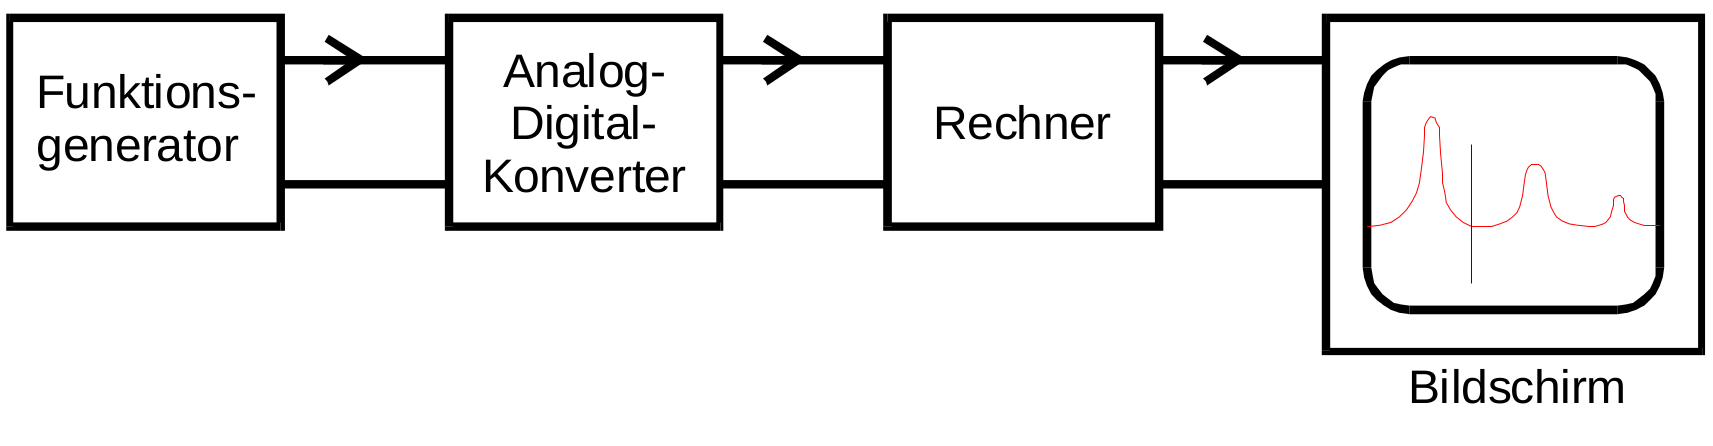
\includegraphics[width=0.4\textwidth]{Analyseschaltung.png}
  \caption{Schaltung für die Fourieranalyse \cite{sample}.}
  \label{fig:Analyseschaltung}
\end{figure}
Es wird mit einem digitalen Oszilloskop eine Fourier-Transormation durchgeführt.
Von diesem werden die ersten $9$ von $0$ verschiedenen Amplituden der Oberwellen
der Analysierten Signale mit dem Cursor abgelesen.
Nun werden die selben Spannungssignale mittels Fourier-Synthese erzeugt. Dafür
wird mit einem Signalgenerator die einzelnen Grund- und Oberwellen erzeugt. Die
Frequenzen werden auf die Verhältnisse der n-ten Oberwelle eingestellt.
Mit den vorher bestimmten Koeffizienten werden die benötigten Amplituden
eingestellt. Mit dem Oszilloskop werden mittels lissajous-Figuren die
Phasendifferenz der einzelnen Oberwellen eingestellt. Dafür wird das Oszilloskop
auf XY-Betrieb gestellt und die Grundwelle mit der einzusellenden Oberwelle
überlagert. Wenn die Synthese abgeschlossen ist, wird das synthetisierte Signal
gespeichert.
